\begin{appendices}
\section{Mind map of elements of Music}
\section{Initial class diagram}
\section{Revised computerised class diagram}
\section{Initial User Interface Design}
\begin{figure}[h]
	\centering
	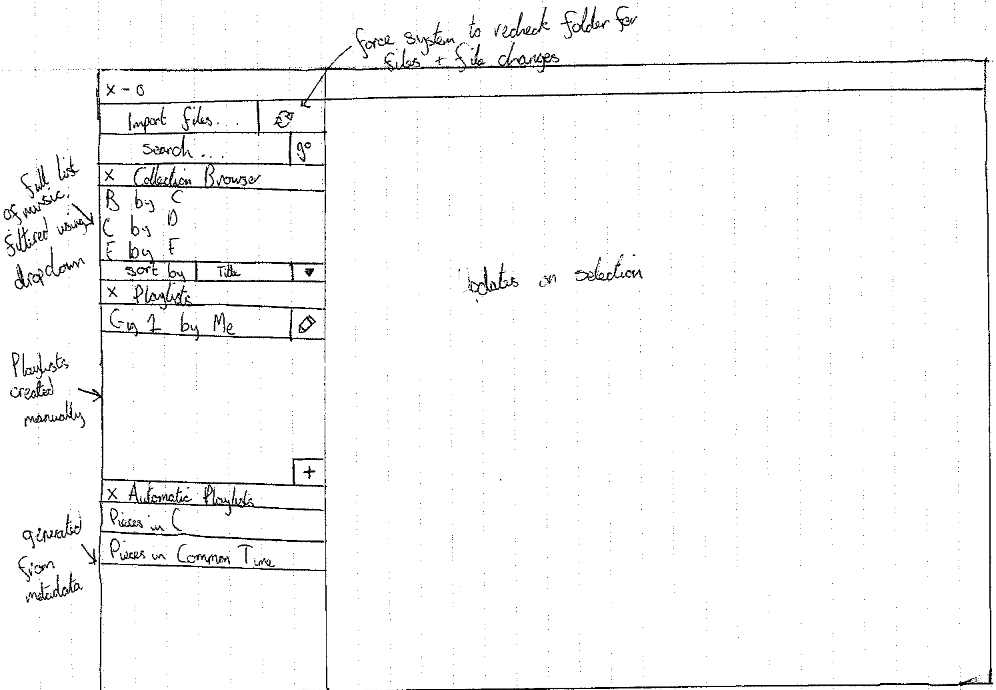
\includegraphics[width=400pt]{designs/main}
	\caption{The main GUI}
	\label{fig:m}	
\end{figure}

Figure ~\ref{fig:m} shows the main graphical user interface. Figure ~\ref{fig:import} shows the popup window displayed when "import files" is clicked. Figure ~\ref{fig:plus} shows the popup window displayed when the plus button on the playlists pane is clicked.
\begin{figure}[H]
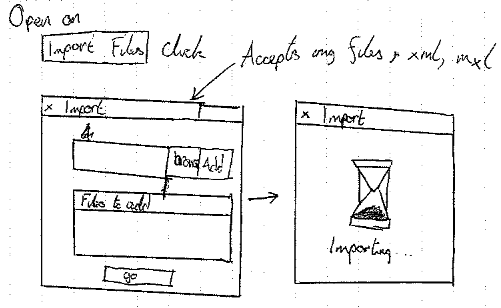
\includegraphics{designs/import_files}
\caption[width=120pt]{Popup box that opens when the user clicks "import files"}	
\label{fig:import}
\end{figure}
\begin{figure}[H]
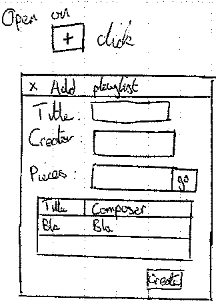
\includegraphics[width=120pt]{designs/create_playlist}
\caption{Popup box on click of the plus button, creating a new playlist}	
\label{fig:plus}
\end{figure}

\subsection{Changes to main display when sheet music selected}
\begin{figure}[H]
	\centering
	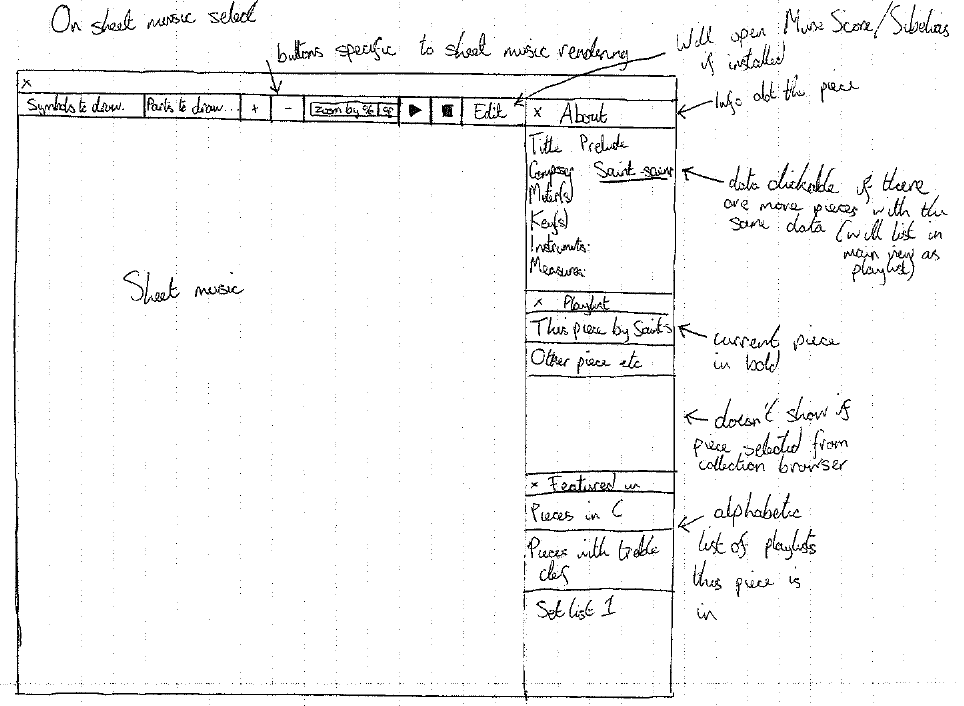
\includegraphics[width=400pt]{designs/sheet_music}
	\caption{The main pane when sheet music is selected}
	\label{fig:sheet}	
\end{figure}
The image shown in figure ~\ref{fig:sheet} shows the updated main pane of figure ~\ref{fig:m} when a piece of music has been selected. The smaller windows to the right show an about pane, which displays all information about the piece itself, a "featured in" pane which will list all playlists containing this piece, and a "playlist" pane. 

Within the about pane, if a piece of data such as "Saint-Saens" in figure ~~\ref{fig:sheet} is underlined, it can be clicked which will lead to a playlist of other pieces which contain the same data.

The playlist pane will only display if the piece has been selected for viewing from an existing playlist. That is to say, if this piece were to be clicked from the collection browser shown in figure \ref{fig:m}, this window would not be open.

\begin{figure}[H]
\begin{minipage}{160pt}
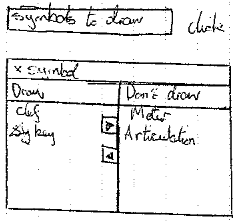
\includegraphics[width=150pt]{designs/symbol_draw}
\caption{The pop up pane displayed when symbols to draw is clicked}	
\label{fig:symbols}
\end{minipage}
\begin{minipage}{160pt}
\centering
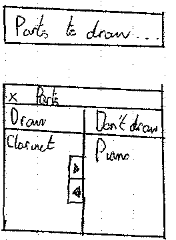
\includegraphics[width=150pt]{designs/part_draw}
\caption{the popup pain displayed when parts to draw is clicked}	
\label{fig:parts}
\end{minipage}
\begin{minipage}{160pt}
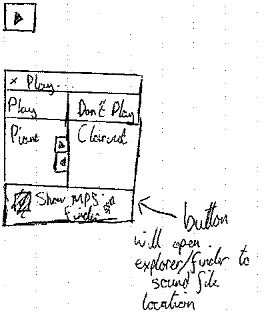
\includegraphics[width=150pt]{designs/play}
\caption{the popup pain displayed when the triangular play button is clicked}
\label{fig:play}
	
\end{minipage}
\end{figure}
The figures \ref{fig:symbols}, \ref{fig:parts}, \ref{fig:play} show the extra windows which display when "symbols to draw", "parts to draw" and the triangle (play) button are clicked, which are buttons displayed above the main pane in figure \ref{fig:sheet}.

\subsection{Changes to main display when playlist is selected}
\begin{figure}[H]
	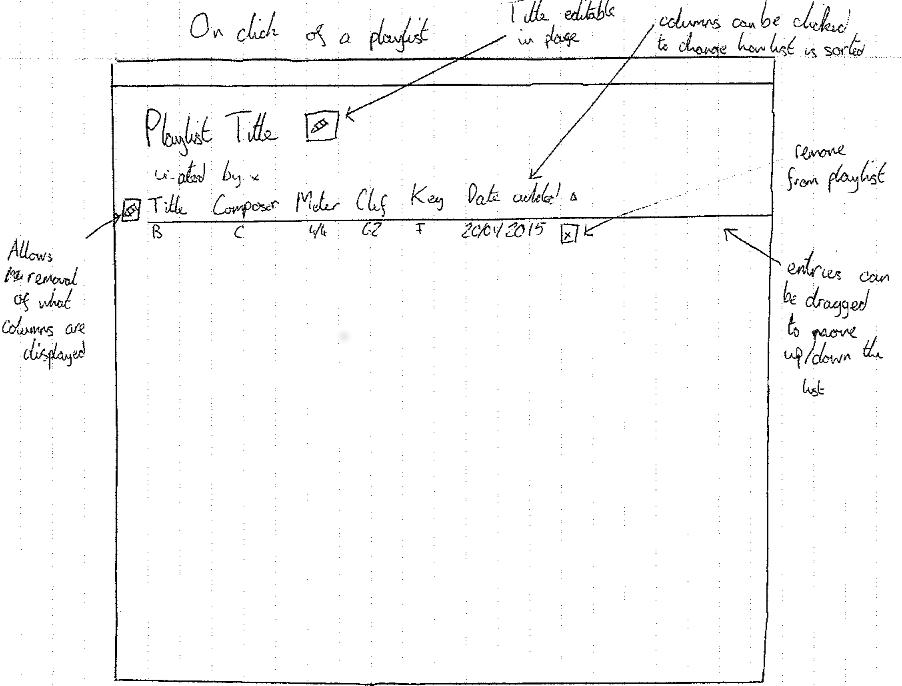
\includegraphics[width=500pt]{designs/playlist}
	\caption{The main pane of the GUI when a playlist is selected}
	\label{fig:playlist}
\end{figure}
Figure \ref{fig:playlist} shows the main pane of figure \ref{fig:m} when a playlist has been selected. This can occur by clicking a manually created playlist from the second pane in figure \ref{fig:m}, an auto-generated playlist from the third pane in the same figure, or by clicking on underlined text in the about pane of figure \ref{fig:sheet}.

The buttons which appear like pens allow the user to edit the title of the playlist or change which columns are displayed - both of these are done in place, that is to say, no extra pop up boxes are needed for the user to change anything in this window. Further to this, the user may move pieces up or down the playlist by dragging the item, and delete them using the "x" button.

\section{User Interface Feedback survey}
\end{appendices}